\chapter{Results and Discussion}\label{ch:eval}
Results for this project were generated using a model that was trained on 1554 regular activity samples. The activities that constitute abnormal data are just falls, and the activities that constituted ADL data are the following:
\begin{itemize}
    \item LayBed
    \item LayFloor
    \item Sit
    \item Background
    \item SitBed
    \item Stand
    \item Transition
    \item Walking
\end{itemize}
The model was trained for 100 epochs, with a window size of 20, and a window step size of 1. A window size of 20 was chosen due to the average length of fall sequences ranging from 20-30 frames. Using a window step size of 1 in conjunction with this window size allows us to generate more contexts and train on more data. With this layout, an activity sample has the following size. 

\begin{center}
$sample\_sequences = \dfrac{total\_frames - window\_size}{window\_step\_size}$    
\end{center}

To test the model, we must first compute a threshold. This threshold is computed using 194 ADL samples and 158 fall samples. To validate the threshold and determine the overall performance of the model, as well as threshold performance, 194 ADL samples, and 158 fall samples, are used.

\section{Results}
\subsection{Model Output}
To display the results of the models' output after the loss function is applied, a histogram was made using the loss values for ADL data and fall data. Figure 4.1a shows the losses for ADL data, Figure 4.1b shows the losses for fall data and Figure 4.2 shows the losses for the fall data put on top of the ADL data.
\begin{figure}[!ht]
\makebox[\linewidth][c]{
    \centering
    \subfloat[\centering ADL losses]{{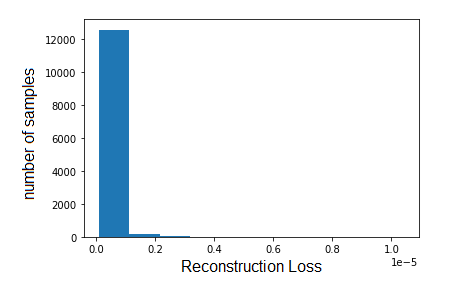
\includegraphics[width=252px, keepaspectratio=true]{adl_losses.png}}}
    \qquad
    \subfloat[\centering Fall losses]{{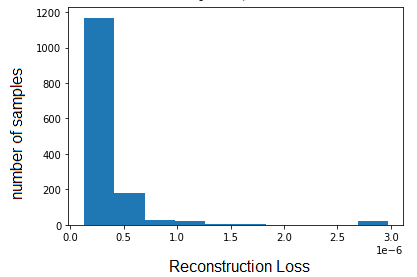
\includegraphics[width=230px, keepaspectratio=true]{fall_losses.png}}}
}
    \caption{Losses from model side by side}
    \label{fig:my_label}
\end{figure}

\begin{figure}[H]
    \centering
    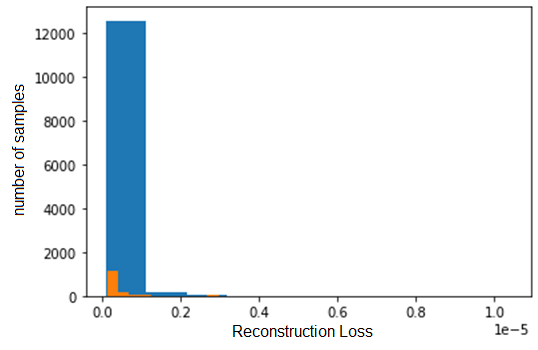
\includegraphics[width=400px, keepaspectratio=true]{combined_losses.png}
    \caption{Fall losses put ontop of ADL losses}
    \label{fig:my_label}
\end{figure}

These results show that there is a much larger (factor of 10) number of frame samples in ADL data in contrast to fall samples. The imbalance of fall samples to ADL samples can be contributed to the rarity of falls in contrast to regular activities. 

Another key result to be noted is that there is a significant overlap between fall losses and ADL losses. This overlap makes it impossible to find an optimal threshold to distinguish between falls and regular activities. Ideally, there would be a clear divide between the fall losses and ADL losses. 

\subsection{Metrics}
To generate the following metrics, 194 ADL samples and 158 fall samples are used. After the threshold is computed using Youden's Index, each sample is checked one at a time. For each sample, we check every single set of frames in the frame sequence, and if any of them are above the threshold, we detect a fall. If the entire sample has losses below the threshold then it is detected as a normal activity. When running this model in real-time it is worth noting that we only handle 1 set of frames at a time for classification. 
\subsubsection{Accuracy}
Table 4.1 gives the model's classification accuracy for falls, ADL data, and combined accuracy. The model accuracy gives an overview of the number of correctly identified samples.

\begin{table}[htp]
    \centering
    \begin{tabular}{ |p{3.5cm}|p{3.0cm}|}
     \hline
     \multicolumn{2}{|c|}{Model Accuracy} \\
     \hline
     Activity& Accuracy\\
     \hline
     \hline
     Falls&40.00\%\\
     \hline
     ADL&41.12\%\\
     \hline
     Total&40.78\%\\
     \hline
    \end{tabular}
    \caption{Model accuracy accross all activities.}
\end{table}
\subsubsection{F1 Score}
When it comes to binary classification, the F1 score gives a deeper insight into model performance. To compute the F1 score, we require the model's precision and recall. Precision as a metric gives the percentage of positive classifications that were actually correct [32]. Model precision is given by the following formula.
\begin{center}
$ Precision = \dfrac{True\_Positives}{True\_Positives + False\_Positives}$
\end{center}

Recall as a metric gives us the percentage of actual positive classifications that were identified correctly [32]. The model recall is computed from the following formula.

\begin{center}
$ Recall = \dfrac{True\_Positives}{True\_Positives + False\_Negatives}$
\end{center}

The F1 score is a combination of precision and recall that aims to give a better idea of the number of incorrectly classified instances in contrast to accuracy. Model F1 score is computed from the following formula. 
\begin{center}
$ F1  Score = \dfrac{2*(Precision * Recall)}{(Precision + Recall)}$
\end{center}

Table 4.2 displays the model's precision, recall, and F1 Score.

\begin{table}[htp]
    \centering
    \begin{tabular}{ |p{3.5cm}|p{3.0cm}|}
     \hline
     \multicolumn{2}{|c|}{F1 Score} \\
     \hline
     Metric& Result\\
     \hline
     \hline
     Precision&26\%\\
     \hline
     Recall&40\%\\
     \hline
     F1 Score&31\%\\
     \hline
    \end{tabular}
    \caption{Model F1 Score}
\end{table}

\subsubsection{ROC Curve}
ROC curves are an excellent metric for determining the performance of a model where a threshold is required. ROC curves allow us to determine how well a model distinguishes between output classes. The curve is a map of the True Positive Rate against the False Positive Rate. The area under the ROC gives a metric to how well the model performed, where 1 is perfect performance. Ideally, the ROC curve follows a logarithmic shape, maximising the area under the curve. Figure 4.3 displays the model's ROC curve.

\begin{figure}[H]
    \centering
    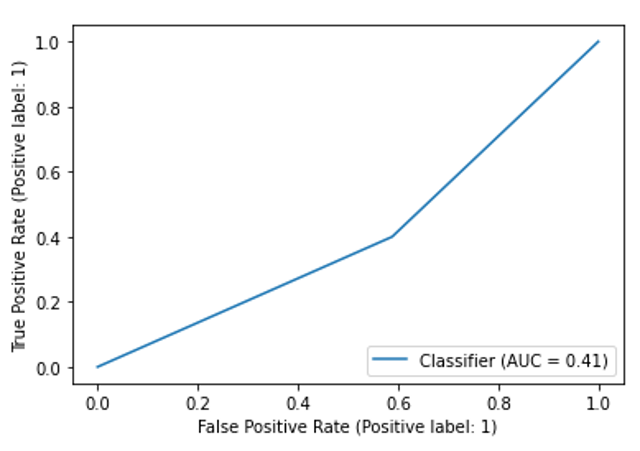
\includegraphics[width=410px, keepaspectratio=true]{roc.png}
    \caption{ROC Curve for model}
    \label{fig:my_label}
\end{figure}

The model developed had an ROC curve that follows the shape of a step function. The step function shifts between two linear functions. The model AUC is 0.41, indicating poor performance.

\subsubsection{Log Loss}
Log-loss is a metric that determines the probability that the prediction is close to the true value. The more the probability diverges from the actual value, the higher the log-loss value [33]. A perfect model has a log-loss score of 0. The higher the log-loss score the worse the performance of the model. The formula to compute log-loss is the following.

\begin{center}
$ Log loss = -\dfrac{1}{N}\sum\limits_{i = 1}^{N}y_i\cdot log(p(y_i)) + (1-y_i)\cdot log(1-p(y_i))$
\end{center}

The current model had a log loss value of 20.45 indicating poor performance of the model.

\section{Evaluation}
\subsection{Outcomes and Analysis}
Through this project, I have developed many scripts and programs that are flexible and simple to work with. I have developed a powerful and specialised data cleaning script that is able to remove noise points, outliers, invalid data points as well as label the data. The data cleaning script is able to create sub-samples out of raw data containing activity data. Alongside this script is a data pre-processing script that groups together points into frame sequences. Connected to these scripts is a detachable variational autoencoder that has capabilities to be run in real-time. With special thanks to Dr. Reza, I was able to develop code for determining an optimal threshold using Youden's Index. The final major outcome of this thesis was determining the underlying issues that severely affected the model's result.

The major takeaway from this project is the versatile and flexible pipeline that was developed. Despite the issues in the data used in this project, the methodology carried out was tested and verified for correctness. The entire process from processing raw data into determining model performance and optimal threshold on a different dataset is as simple as changing the dataset.

The model had performed poorly in distinguishing falls from ADL activities. However, this issue can be attributed to a poor dataset, and in any machine learning project, your model is as good as the data it has to work with. When compared with other models developed by colleague Nathan Ng, the accuracy had only differed by 2\%. The same models developed had performed exceptionally well when used on different datasets. Whilst the issue could be that this approach is unrealistic for the detection of falls and the model performs poorly, it is more likely that the issue lays inside of the dataset.
\subsection{Data Issues}
When performing a in-depth look into the dataset major issues had emerged that were not taken into consideration during data collection. This project had been reliant on this dataset and worked under the assumption that the data was not problematic. 
\subsubsection{Target Tracking}
Target tracking is a crucial step in determining which point belongs to which entity. In the samples since there is only one person in the scene, we expect that there is only one target that is being tracked. However when observing the dataset it can be noted that multiple targets are being detected. Figure 4.4 displays the issue of multiple targets being tracked.

\begin{figure}[H]
    \centering
    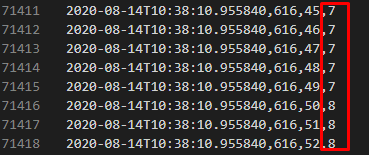
\includegraphics[width=300px, keepaspectratio=true]{multiple_targets.png}
    \caption{Multiple target id's when only one target in scene.}
    \label{fig:my_label}
\end{figure}

Alongside having multiple targets detected, the synchronisation between the target id file and raw point data file are inconsistently out of sync. In some cases, the target id file would be missing up to 50,000 points, meaning those points could not be linked to any target or determined to be noise. Figure 4.5 shows the large disparity between the track id file and point cloud file.

\begin{figure}[H]
    \centering
    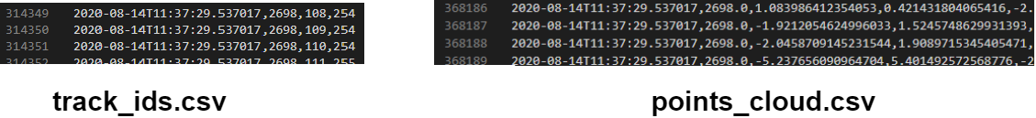
\includegraphics[width=380px, keepaspectratio=true]{badsync.png}
    \caption{50,000 points missing from track id file.}
    \label{fig:my_label}
\end{figure}

Additionally, for certain subjects, there would be a random amount of rows being tracked in the track id file, and suddenly a new sample would begin in the same file. This inconsistency makes it impossible to determine which point belongs to which target. In figure 4.6 the track id file has tracked the first 616 frames, and suddenly a new header row is inserted (had to be manually deleted) and the sample starts again from frame 1. This kind of inconsistency makes it unclear how to approach noise removal.  

\begin{figure}[H]
    \centering
    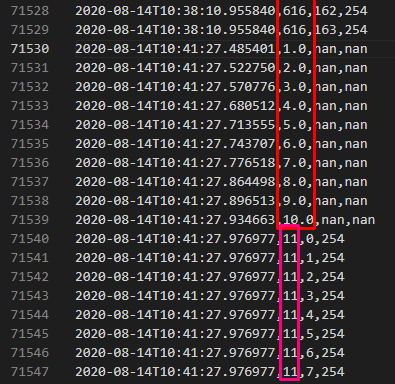
\includegraphics[width=250px, keepaspectratio=true]{junkrows.png}
    \caption{Random restart in track id file 71,529 rows in.}
    \label{fig:my_label}
\end{figure}

Finally, missing frames were present in the points cloud csv files. This is another inconsistent issue that occurs randomly in some samples, where there would be a missing frame in the points cloud file but the same frame is being tracked in the track id file. Figure 4.7 shows a sample where frame 243 is missing however frame 243 can be found in the track id file.
\begin{figure}[H]
    \centering
    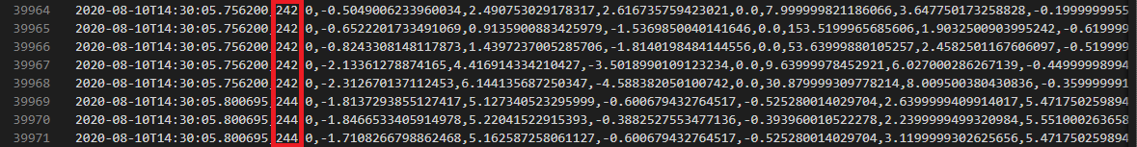
\includegraphics[width=450px, keepaspectratio=true]{missing_frames.png}
    \caption{Frame 243 missing from the sample.}
    \label{fig:my_label}
\end{figure}

\subsubsection{Noise Removal}
An enormous chunk of the data was attributed to noise. Around 80\% of all points were classified as noise when determining the track ids. The removal of this noise created a largely sparse dataset and displayed quite some strange results. In appendix 1, a sequence of images displays the severity of the noise removal when it comes to this dataset. The first two images in appendix 1 show the contrast between noise removal correctly working and noise removal not working entirely. Following is a sequence of images showing frames that are classified as falls after having noise removal performed on them. These frames are in sequential order from one fall sample. As shown in appendix 1, it would randomly switch between correctly removing noise and being unable to distinguish noise. 

The inability to consistently determine noise from regular data, alongside 80\% of the data being noise itself, makes it impossible to achieve meaningful results.

\subsection{What Could of Been Different}
When looking back to thesis A, it was clear I was not checking back on my work as often as I should have. When developing complex algorithms and specific scripts, it is important to take a step back to ask yourself what are you doing, and make sure you're on the right track. Had I understood the data earlier on and done more work with the data, the entire scope of my project may have changed altogether. The data issues came to life in thesis C when trying to analyse my results for the first time. The final change I would have made going back would have been to manage my time better to get more out of this project. Often I would find myself stuck on specific issues that did not have an obvious solution. In these situations, it would have been better to ask my supervisor for help or consider alternative approaches instead of forcing certain solutions to work. 